\documentclass[12 pt]{article}
%%%%%%%%%%%%%%%%%%%%%%%%%%%%
%\topmargin 0.2in
%\textheight 10in
%\voffset -1.25in
%\textwidth 6.2in
%\parindent 0.25in
%\itemindent 0.in
%\leftmargin 0.5in
%\hoffset -0.8in




%Packages
\usepackage{graphicx}
\usepackage[mathcal,mathscr]{eucal}
\usepackage{amsfonts}
\usepackage{mathrsfs}
\usepackage{amsmath, amsthm, amssymb,epsfig,amscd,multicol}
\usepackage{enumitem}
\usepackage{xcolor}
\usepackage{tikz}
\usetikzlibrary{arrows,positioning,shapes,fit,calc}
\usepackage{float}
\usepackage{caption}
\usepackage{subcaption}
\usepackage[style=1]{mdframed}
%\usepackage{tabu}
\usepackage{arydshln}
\usepackage{cancel}
\usepackage[margin=2cm,top=1.5cm]{geometry}
%\usepackage{mathptmx}

%New Commands
\newcommand{\R}{\mathbb{R}}
\newcommand{\Z}{\mathbb{Z}}
\newcommand{\Q}{\mathbb{Q}}
\newcommand{\N}{\mathbb{N}}
\renewcommand{\P}{\mathscr{P}}
\newcommand{\set}[1]{\left\{#1\right\}}
\newcommand{\ds}{\displaystyle}
\newcommand{\diff}[2]{\frac{d #1}{d #2}}
\renewcommand{\subset}{\subseteq} 
\newcommand{\divides}{\! \mid \!}
\newcommand{\ndivides}{\! \nmid \!}
\newcommand{\mymod}[1]{ \ (\bmod \ #1)}
\newcommand{\esub}{\subseteq}
\newcommand{\rel}{\mathbin{R}}

\theoremstyle{definition}
\newtheorem{remark}{Remark}

\theoremstyle{plain}

\newtheoremstyle{mytheorem}% name of the style to be used
  {6pt}% measure of space to leave above the theorem. E.g.: 3pt
  {6pt}% measure of space to leave below the theorem. E.g.: 3pt
  {\itshape}% name of font to use in the body of the theorem
  {0pt}% measure of space to indent
  {\bfseries}% name of head font
  {.}% punctuation between head and body
  {5 pt plus 1pt minus 1pt}% space after theorem head; " " = normal interword space
  {}% Manually specify head
  
 	\theoremstyle{mytheorem}
  	\newtheorem{theorem}{Theorem}[section]%[numbering]
	\newtheorem{lemma}{Lemma}
	\newtheorem{cor}{Corollary}[section]
	
	

\newtheoremstyle{myexample}% name of the style to be used
  {22pt}% measure of space to leave above the theorem. E.g.: 3pt
  {22pt}% measure of space to leave below the theorem. E.g.: 3pt
  {\normalfont}% name of font to use in the body of the theorem
  {0pt}% measure of space to indent
  {\bfseries}% name of head font
  {.}% punctuation between head and body
  {5 pt plus 1pt minus 1pt}% space after theorem head; " " = normal interword space
  {}% Manually specify head

	\theoremstyle{myexample}
	\newtheorem{example}{Example}[section]
	\newtheorem{claim}{Claim}
	
	
\newtheoremstyle{mydefinition}% name of the style to be used
  {12pt}% measure of space to leave above the theorem. E.g.: 3pt
  {12pt}% measure of space to leave below the theorem. E.g.: 3pt
  {\normalfont}% name of font to use in the body of the theorem
  {0pt}% measure of space to indent
  {\bfseries}% name of head font
  {.}% punctuation between head and body
  {5 pt plus 1pt minus 1pt}% space after theorem head; " " = normal interword space
  {}% Manually specify head

	\theoremstyle{mydefinition}
	\newtheorem{definition}{Definition}
	\newtheorem*{definition*}{Definition}





\begin{document}
\pagenumbering{gobble}
\begin{center}
\textbf{Logical Problem Solving and Arguments}
\end{center}

%We're not ready to write proofs just yet.  We haven't discussed what a proof really is, nor what makes a proof good or bad.  However, you're at a point of mathematical maturity where you are capable of explaining your reasoning when you solve problems.  These explanations are in fact arguments based on known mathematical techniques and logic.  As we progress in this course, you will turn these arguments into the foundations of your proofs.\\
%
%  In the following exercises, your goal is to provide an argument, based on the given definitions, that the statement is true.  The following definitions aren't perfect, but they will work for now.  Below, the collection of integers is denoted by $\mathbb{Z}$.
%\begin{center}
%\fbox{\parbox{5.5in}{Goals:
%\begin{itemize}
%\item Provide arguments to simple mathematical ideas based on provided definitions
%\item Articulate arguments so that they can be understood by any audience
%\end{itemize}
%}}
%\end{center}
%
%
%
%%\begin{center}
%%\fbox{\parbox{6in}{
%%\begin{definition}[Even]  An integer $n$ is \textit{even} if $n=2k$ for some $k \in \mathbb{Z}$.
%%\end{definition} 
%%
%%\begin{definition}[Odd] An integer $n$ is \textit{odd} if it is not even.
%%\end{definition}
%%}}
%%\end{center}
%
%\begin{enumerate}
%\item Suppose that $n$ and $m$ are even integers.  Explain why $n+m$ must be an even integer.
%
%\item Suppose that $n$ is an even integer and $m$ is an odd integer.  Explain whey $n+m$ must be an odd integer.
%\end{enumerate}

%\begin{center}
%\fbox{\parbox{6in}{
%\begin{definition}[Even]  A function $f$ is \textit{even} if $f(-x) = f(x)$ for all $x$ in the domain of $f$.
%\end{definition}
%\begin{definition}[Odd]  A function $f$ is \textit{odd} if $-f(x)=f(-x)$ for all $x$ in the domain of $f$.
%\end{definition}
%}}
%\end{center}
%
%\begin{enumerate}
%\setcounter{enumi}{2}
%\item Let $f(x)=x^2+4$ and $g(x)=(x-1)^2$.  Explain how know that $f$ is even while $g$ is not.  Does this mean that $g$ is odd?
%\end{enumerate}

Being able to write proofs opens up your mind to being able to systematically solve general problems.  Not only will you be able to reason your way through and solve the given problem, you will be able to explain how you \textit{know} you have a correct solution.  The following problems are not \textit{math} problems; they are \textit{logic} problems.  You need a clear head and careful thought to solve them, not knowledge from a prior math class.\\

\begin{center}
\fbox{\parbox{5.5in}{Goals:
\begin{itemize}
\item Analyze simple problems not based on given examples
\item Solve problems with no algorithm provided
\item Argue that solutions are valid
\end{itemize}
}}
\end{center}


\begin{enumerate}
\item (Needy Children)  Mrs.~Jones has twin girls.  When out shopping the family comes across a gum ball machine which offers red gum balls and purple gum balls.  The savvy Mrs.~Jones knows that she has to give the same color gum ball to each twin to ensure that no one throws a fit.  What is the maximum number of gum balls that Mrs.~Jones must purchase to ensure that each twin has the same color gum ball?  After working out the maximum number, provide a carefully developed argument explaining how you know this is the correct answer.

%\item (Super-Simple Nim)  Nim is a classic game with a lot of mathematical implications.  The rules vary and can be complicated, but we'll just consider a simple version.  The game consists of two players and a pile of four stones.  Players take turns removing stones from the pile.  On his or her turn, a player may remove either one or two stones.  The goal of the game is to be the person to pick up the last stone.  Is there an optimal strategy for the first player?  That is, can Player 1 start the game with a move that will guarantee a win no matter what choices Player 2 makes?  If you find an optimal strategy, provide a carefully developed argument that explains how you know Player 1 always wins using this strategy.  Your explanation should include how know this is the optimal strategy.

\item (The King's Fortress)  A king wants to design fortress with 10 towers and walls running between the towers.  The king wants 4 towers on each wall and wants as many towers surrounded by walls as possible.  One of the king's servants suggests the following arrangement.
\begin{center}
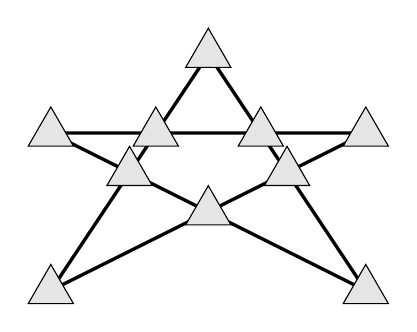
\begin{tikzpicture}[main node/.style={regular polygon,regular polygon sides=3,fill=gray!20,draw,minimum size=0.5cm}]
\draw[very thick] (-2,0)--(0,3)--(2,0)--(-2,2)--(2,2)--(-2,0);
\node[main node] at (-2,0){};
\node[main node] at (0,3){};
\node[main node] at (2,0){};
\node[main node] at (-2,2){};
\node[main node] at (2,2){};
\node[main node] at (-.66666,2){};
\node[main node] at (-1,1.5){};
\node[main node] at (0,1){};
\node[main node] at (.66666,2){};
\node[main node] at (1,1.5){};
\end{tikzpicture}
\end{center}

%\begin{center}
%\begin{tikzpicture}[->,>=stealth',shorten >=1pt,auto,node distance=1cm,
%        thick,main node/.style={regular polygon,regular polygon sides=3,fill=gray!20,draw,minimum size=0.5cm,inner sep=0pt]}]
%
%    \node[main node] (1) {};
%    \node[main node] (2) [below left of=1]  {};
%    \node[main node] (3) [below right of=1] {};
%    \node[main node] (4) [left of=2] {};
%    \node[main node] (5) [right of=3]{};
%    \node[main node] (6) [below left of=2]{};
%    \node[main node] (7) [below right of=3]{};
%    \node[main node] (8) at ([shift={(0,-2)}]1) {};
%    \node[main node] (9) [below left of=6]{};
%    \node[main node] (10) [below right of=7]{};
%
%    \path[-]
%    (1) edge node {} (2)
%        edge node {} (3)
%    (2) edge node {} (1)
%        edge node {} (3)
%        edge node {} (6)
%        %edge node {} (8)
%    (3) edge node {} (1)
%        edge node {} (2)
%        edge node {} (7)
%     (4) edge node {} (2)
%     		edge node {} (6)
%	(5) edge node {} (3)
%		edge node {} (7)
%	(6) edge node {} (9)
%		edge node {} (8)
%	(8) edge node {} (9)
%		edge node {} (7)
%	(10) edge node {} (8)
%		edge node {} (7);
%\end{tikzpicture}
%\end{center}
This meets the requirement for the walls, but none of the towers are contained entirely within walls.  Give a better arrangement.

\item (Jelly Bean Mix-Up)  You are presented with three jelly bean jars.  One jar contains cherry flavored beans, another contains orange flavored beans, and the third contains a mix of cherry and orange.  Each jar is labeled, but the labels are \textit{all wrong}.  What is the minimum number of jelly beans you must eat to properly correct the labels?  After working out the minimum number, provide a carefully developed argument explaining how you know this to be the correct solution.

\item (Lost in the Woods)  You are driving to a very important meeting and you realize that you're going to be late.  Your GPS tells you that you can take a short cut through the woods that will get you there on time.  You quickly check the route and notice that it consists of a single road through the woods, so you decide to take it since you can't get lost.  An hour into the woods you come to a fork in the road with no signs.  You've lost your GPS signal, so you realize that you'll need to ask for directions.  Fortunately, there is an inn at the fork in the road.  As you walk up to the inn, you notice a sign on the front door that says the following.
	\begin{center}\parbox{5in}{Two identical twin brothers live here and they can give you directions.  However, you may only ask them one question per day and it will only be answered by the twin to which you address the question.  One of the twins always lies, the other always tells the truth, and you can't tell them apart.
	}

	\end{center}
	There is exactly one question that you can ask the twins that will help you.  What is that question and how do you use the answer to get to the meeting on time?

\item (A Burning Problem) You are given two ropes that take exactly 60 minutes each to burn.  The lengths of the ropes burn inconsistently, meaning that it's possible for half the rope to burn in a few seconds and the other half to take nearly an hour.  Find a way to use the two ropes to measure 45 minutes.  Provide a carefully written explanation of how you know your solution is correct.

\item (Find the Fake). You are given 7 gold coins that appear to be identical, but one is a fake and weighs slightly less than the other 6.  You are also given a balancing scale.  Find a way to determine which coin is that fake by using the scale \textit{only twice}.  Give a carefully written explanation of your solution.

\end{enumerate}
\end{document}




